\section{Use Case Specification for Actor: Jockey}
\label{sec:srs_jockey}

In the Horse Racing Tournament Management System, the interaction flow between the Horse Owner and the Jockey represents a core business logic workflow. This section focuses specifically on the selection and invitation process of a Jockey, covering the primary actions where a Horse Owner extends a formal invitation, and the Jockey subsequently reviews and either accepts or declines it.

\subsection{Activity Diagram}

The activity diagram below illustrates the comprehensive step-by-step operational workflow of the system. To maintain strict data integrity, the system is designed to securely persist the invitation status in the database prior to executing the notification dispatch layer to the targeted Jockey.

\begin{figure}[htbp]
	\centering
	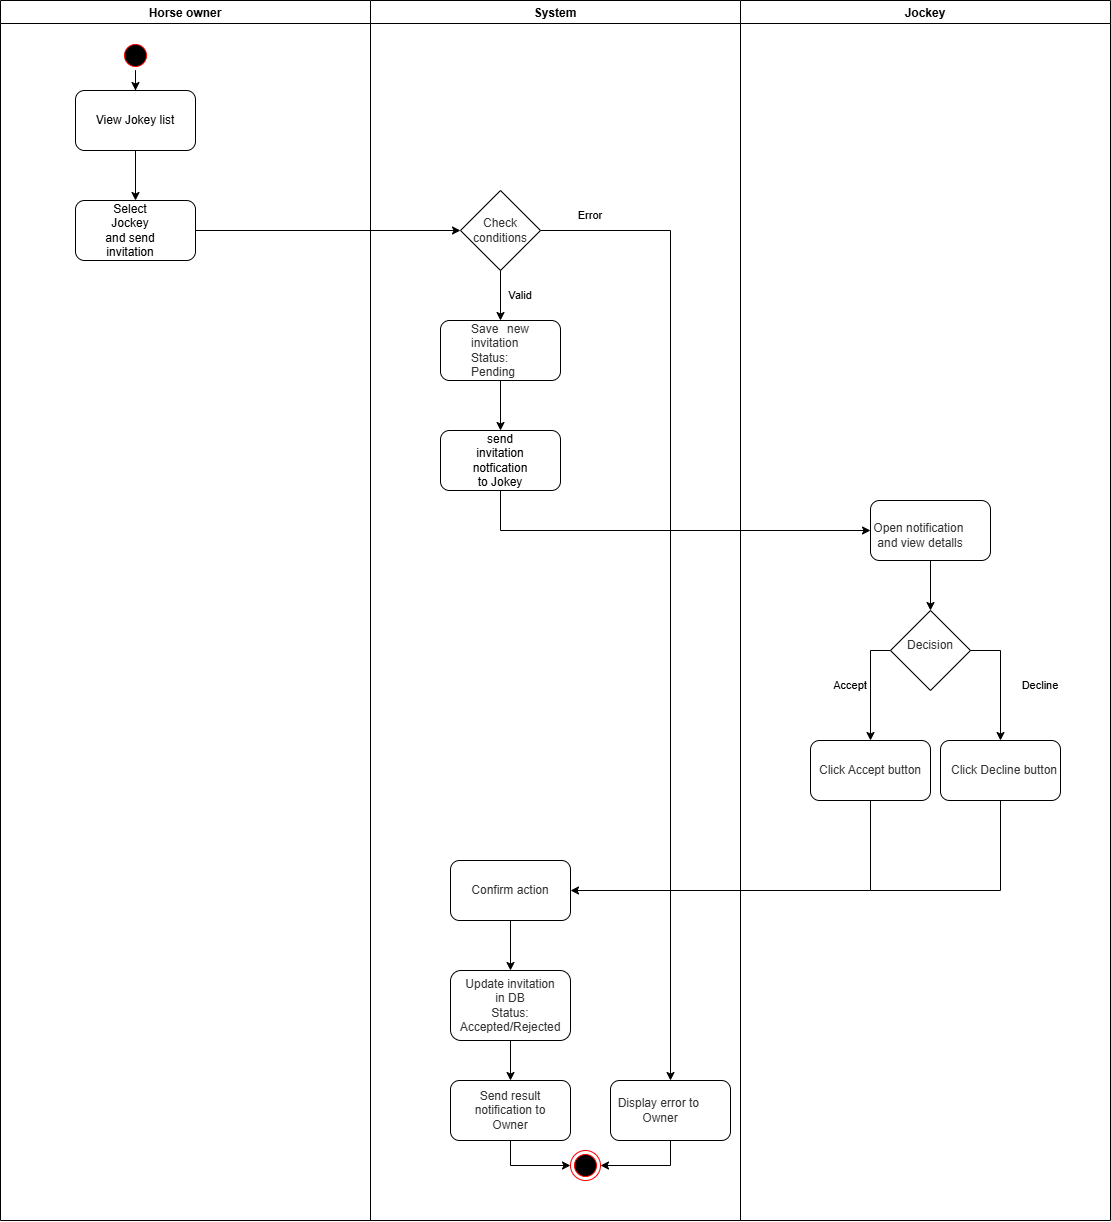
\includegraphics[width=0.9\textwidth,height=0.75\textheight,keepaspectratio]{images/chuong3/activity_jockey.png}
	\caption{Activity Diagram: Jockey Invitation and Confirmation Process}
	\label{fig:activity_jockey}
\end{figure}

As visualized in Figure~\ref{fig:activity_jockey}, the workflow initiates as soon as the Horse Owner triggers an invitation request.

\subsection{Sequence Diagram}

The sequence diagram provides a detailed technical view of the chronological message exchanges and method invocations between the active architectural objects within the system.

\begin{figure}[htbp]
	\centering
	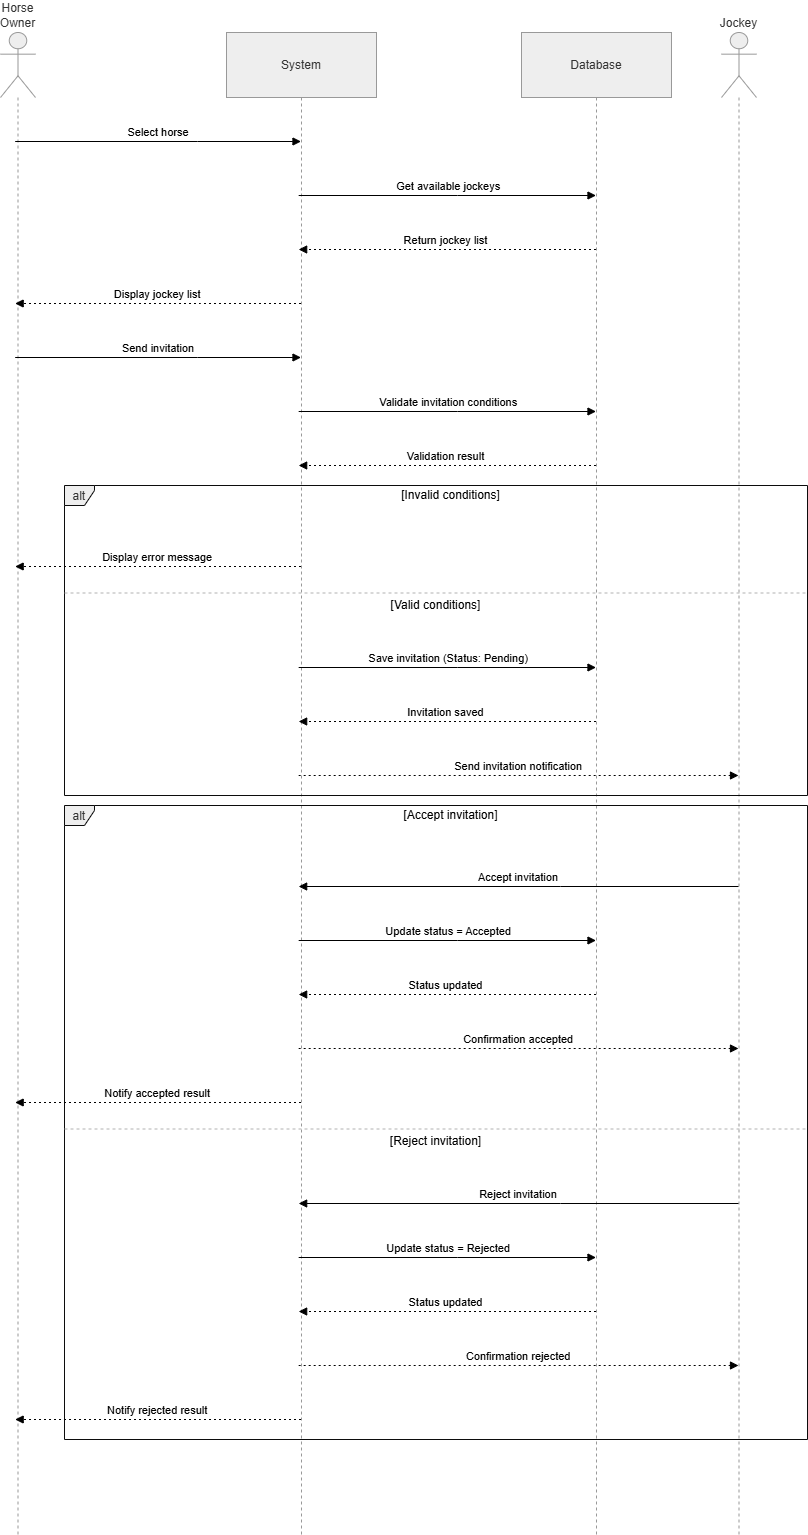
\includegraphics[width=0.9\textwidth,height=0.75\textheight,keepaspectratio]{images/chuong3/sequence_jockey.png}
	\caption{Sequence Diagram: Jockey Invitation and Confirmation Process}
	\label{fig:sequence_jockey}
\end{figure}

Figure~\ref{fig:sequence_jockey} maps out the explicit timeline and reactive logic of the transactional interactions.

\subsection{Screen Flow}

The screen flow captures the practical user interface navigation layout that both the Horse Owner and the Jockey will interact with to complete this use case successfully.

\begin{figure}[htbp]
	\centering
	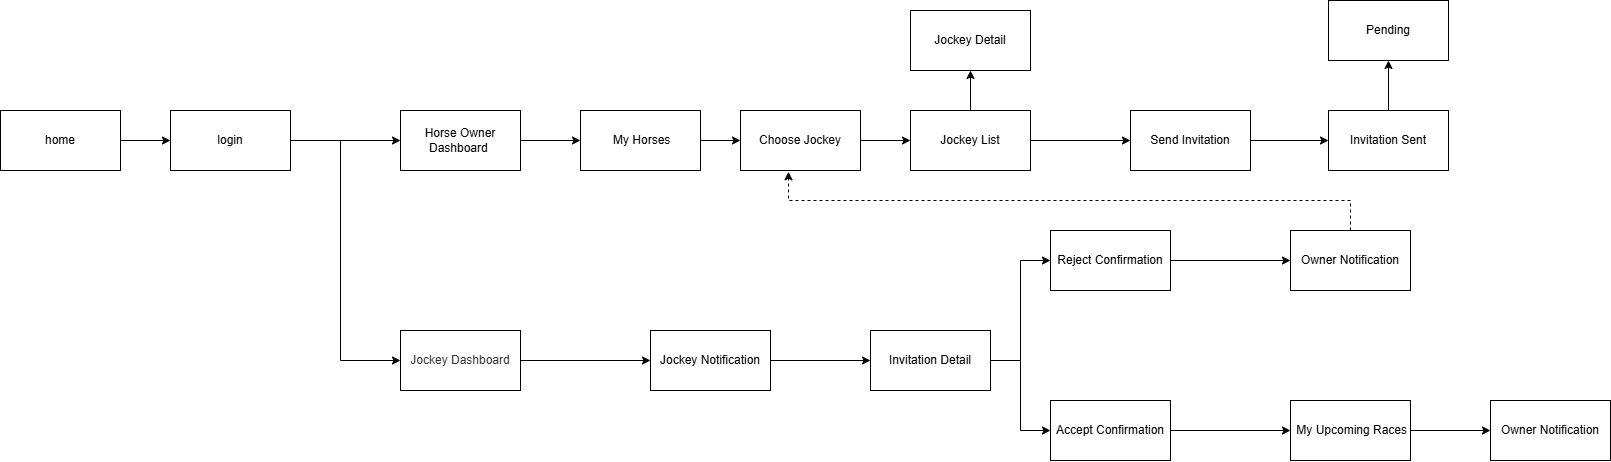
\includegraphics[width=0.9\textwidth,height=0.75\textheight,keepaspectratio]{images/chuong3/screenflow_jockey.png}
	\caption{Screen Flow: Jockey Invitation Management Interface}
	\label{fig:screenflow_jockey}
\end{figure}

Based on the interface mapping in Figure~\ref{fig:screenflow_jockey}, users can seamlessly transition across the functional layout.